The underlying event measurement in p+p collisions is performed using the calorimeter towers as the basic input for the measurement.
The calorimeter towers are reconstructed using the nominal calorimeter calibration and reconstruction procedure outlined in Section~\ref{sec:nominal_calorimeter_reconstruction}.
The calorimeter towers are clustered into jets using the anti-$k_{T}$ algorithm with a radius parameter of R = 0.4 without underlying event subtraction~\cite{jetreco_macro}. 
The reconstruction details for the anti-$k_{T}$ algorithm are included in Section~\ref{sec:jet_algo}.
The calorimeter towers are also clustered into topoclusters using the default sPHENIX topocluster reconstruction parameters~\cite{topo_macro}.
A detailed description of the topocluster algorithm, reconstruction and optimization for this analysis is included in the following sections.

\subsection{Topocluster algorithm}

The calorimeter topoclustering algorithm groups individual calorimeter towers into clusters and is designed to reconstruct electromagnetic and hadronic showers as cluster objects.
Topoclusters are an ideal clustering method when looking to suppress electronic noise and pile-up contributions. 
To limit these noise contributions, the clustering algorithm requires energies much higher than the noise floor for seeding and expanding clusters.~\cite{ATLAS:2017_topological_cluster_performance,ATLAS:2024_topological_cluster_timing}. 
Topoclusters are grown using the following thresholds:
\begin{itemize}
    \item Seed threshold ($S$): Towers with $|E_{\mathrm{tower}}| > S\,\sigma_{\mathrm{noise}}$ initiate clusters, where $S=4$.
    \item Neighbor growth threshold ($N$): Adjacent towers with $|E_{\mathrm{tower}}| > N\,\sigma_{\mathrm{noise}}$ added to expand the cluster, where $N=2$.
    \item Peripheral threshold ($P$): Boundary towers bordering the neighboring towers, where $P=0$.
\end{itemize}
where each threshold is defined in units of the tower noise: $\sigma_{\mathrm{noise}}$.

Topoclusters are grown outwards from seed towers using towers adjacent in either $\eta$ or $\phi$ within the same calorimeter layer or overlapping in the $(\eta,\phi)$ plane across layers (EMCal, IHCal, and OHCal). These neighboring towers must satisfy the $N$ threshold to be added to the cluster and can then itself seed further neighbors, expanding the cluster until no additional towers meet the $N$ criteria. 
After this, boundary towers at the $P$ threshold are then included to preserve the full shower shape with minimal noise contamination.
An example of topocluster growth is shown in the distribution of topoclusters across calorimeter layers in a simulated dijet event display (Figure~\ref{fig:topocluster_event_display}). 

\begin{figure}
    \centering
    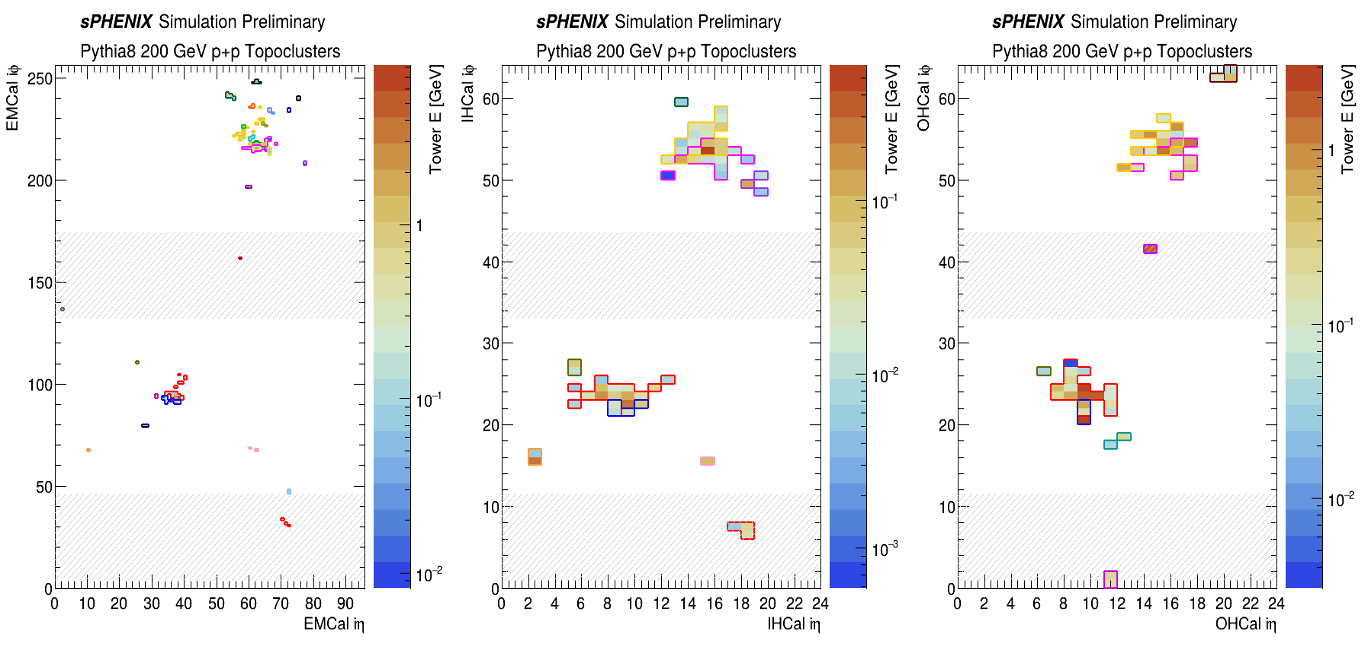
\includegraphics[width=\linewidth]{figures/chapter5/topocluster_event_display.png}
    \caption{Display of topocluster boundaries (colored line borders) across the EMCal (left), IHCal (middle) and OHCal (right) calorimeter layers for a dijet event in $p+p$ collisions in \pythia. Each panel shows a rolled-out projection of the calorimeter acceptance, with the tower pseudorapidity index $i\eta$ on the horizontal axis and the tower azimuthal index $i\phi$ on the vertical axis. Tower energies in GeV are indicated by the fill color, with the scale shown by the color axis on the right. The transverse region is shown in gray shading.}
    \label{fig:topocluster_event_display}
\end{figure}

\subsection{Setting topocluster noise thresholds}
Topocluster noise thresholds are optimized for the calorimeter noise conditions during the Run 2024 $p+p$ running.
First, the tower-by-tower pedestal RMS for each calorimeter layer is determined from pedestal data. These tower-by-tower pedestal RMS values are shown in Figure~\ref{fig:pedestal_RMS}. The means of these tower-by-tower pedestal RMS are extracted for each of the calorimeters from these plots. The EMCal mean RMS = 30.4 MeV, the IHCal mean RMS = 1.77 MeV, and the OHCal mean RMS = 11.7 MeV.

From previous studies of changes in the calorimeter noise across the p+p running~\cite{calo_noise_run2}, it is known that the EMCal noise increased across the p+p running while the IHCal and OHCal noise stayed fairly constant. Therefore, the pedestal data used to determine the tower-by-tower pedestal RMS, taken directly after the $p+p$ beam running, is a slight overestimate of the EMCal average noise across the full Run 2024 p+p running period. In the nominal $p+p$ simulation production, a scaling factor of 0.75 is applied to the pedestal noise fluctuations so that the simulation matches the pedestal region of beam runs from the full Run 2024 p+p data. This same scaling factor of 0.75 is applied to the EMCal mean pedestal RMS for consistency, giving an EMCal mean pedestal RMS of 22.8 MeV during the 2024 p+p running. 

Now with accurate values for the pedestal effects in each of the calorimeters during the 2024 p+p running, truth particle to topocluster matching is tested for two, three and four times the mean pedestal RMS values of the calorimeter layer using a minimum-bias \pythia simulation sample with realistic pedestal noise embedded. The topocluster sensitivity to noise is tested by finding the relative width of the $E/p$ distributions for topoclusters matched to truth particles. More details on this method are included in the next section, Section~\ref{sec:topo_resolution}. 
The full set of tested pedestal RMS values are included in Table~\ref{tab:topo_noise_parameters}. 
\begin{table}[]
    \centering
    \begin{tabular}{c|c|c|c|c|c}
        Calorimeter & Pedestal run $\langle \sigma_{ped} \rangle$ & p+p running $\langle \sigma_{ped} \rangle$ & p+p $\langle 2\sigma_{ped} \rangle$ & p+p $\langle 3\sigma_{ped} \rangle$ & p+p $\langle 4\sigma_{ped} \rangle$ \\
        \hline
        EMCal & 30.4 & 22.8 & 45.6 & 68.4 & 91.2 \\
        IHCal & 1.77 & 1.77 & 3.5 & 5.3 & 7.0 \\
        OHCal & 11.7 & 11.7 & 23.4 & 35.1 & 46.8 \\
    \end{tabular}
    \caption{Table of pedestal RMS values extracted and used as topocluster noise parameters for p+p running. All $\sigma_{ped}$ values are given in MeV.}
    \label{tab:topo_noise_parameters}
\end{table}

\begin{figure}
    \centering
    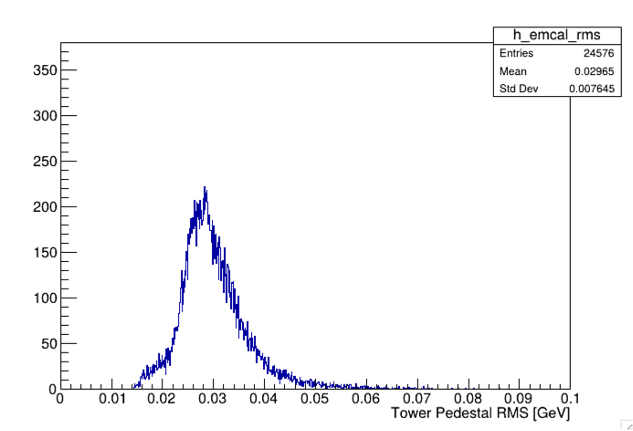
\includegraphics[width=0.48\linewidth]{ueinpp/Figures/topocluster_noise/emcal_pedestal_rms.png}
    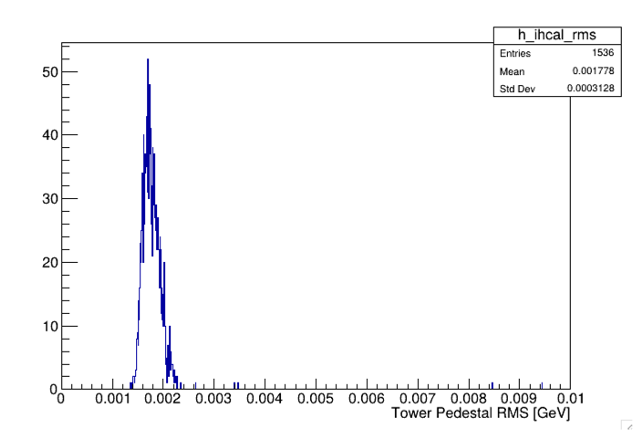
\includegraphics[width=0.48\linewidth]{ueinpp/Figures/topocluster_noise/ihcal_pedestal_rms.png}
    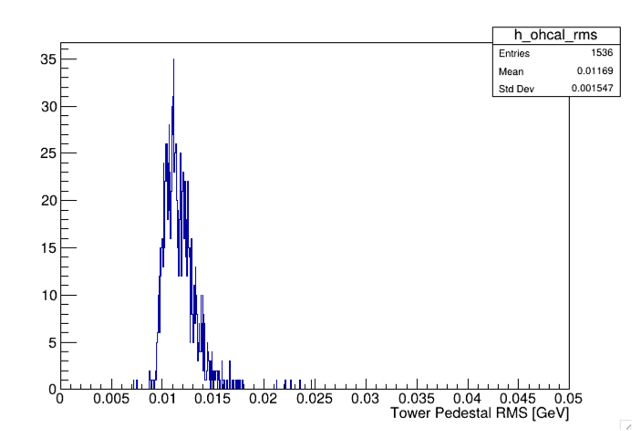
\includegraphics[width=0.48\linewidth]{ueinpp/Figures/topocluster_noise/ohcal_pedestal_rms.png}
    \caption{Tower-by-tower pedestal RMS for EMCal (top left), IHCal (top right) and OHCal (bottom) found from pedestal data. Mean RMS is extracted, scaled to match pedestal in beam data, and used for testing noise thresholds in topocluster seeding.}
    \label{fig:pedestal_RMS}
\end{figure}

\subsection{Topocluster resolution}
\label{sec:topo_resolution}

The resolution of topoclusters is studied in the \pythia p+p simulation with realistic embedded pedestal noise and separately for electromagnetic (EM) and hadronic particles. For EM particles, $\gamma$ and $e^{\pm}$, truth particles with $E>1$\,GeV are matched to clusters within $\Delta R<0.1$, while for hadronic particles, $\pi^{\pm}$, truth particles with $E>3$\,GeV are matched within $\Delta R<0.2$. 
The resolution is quantified using the relative width of the $E/p$ ratio, where $E$ is the topocluster energy and $p$ is the momentum of the matched truth particle.  
Since this study was conducted in a minimum bias collision event instead of a single-particle simulation, an isolation condition is applied, requiring the truth particle to have no other nearby truth particles with transverse momentum $p_T > 0.2$\,GeV within a cone of $\Delta R < 0.6$. 

The analysis is performed for the three noise suppression thresholds: $\langle2\sigma_{ped}\rangle$, $\langle3\sigma_{ped}\rangle$, and $\langle4\sigma_{ped}\rangle$. The explicit values for these noise threshold are given in Table~\ref{tab:topo_noise_parameters} and the methodology for determining these values is outlined in the above section. These thresholds are used to evaluate how noise impacts the resolution performance of topoclusters.

The extracted resolutions from the $E/p$ distributions for EM particles are 13.7\%, 13.4\%, and 13.3\% for the $\langle2\sigma_{ped}\rangle$, $\langle3\sigma_{ped}\rangle$, and $\langle4\sigma_{ped}\rangle$ thresholds, respectively. 
While the extracted resolutions for the $E/p$ distributions for hadronic particles are 69.1\%, 59.6\%, and 58.9\% for the $\langle2\sigma_{ped}\rangle$, $\langle3\sigma_{ped}\rangle$, and $\langle4\sigma_{ped}\rangle$ thresholds, respectively.  
While the resolutions are very similar for the EM shower case, in the hadronic shower case, the resolutions obtained with the $\langle3\sigma_{ped}\rangle$ and $\langle4\sigma_{ped}\rangle$ thresholds are better than the resolution from the $\langle2\sigma_{ped}\rangle$ threshold and are found to be very similar to each other. 
Therefore, the $\langle3\sigma_{ped}\rangle$ threshold is selected for the nominal topocluster reconstruction threshold in the analysis.
Figure~\ref{fig:topocluster_resolution_3sigma} shows the $E/p$ distributions for the $\langle3\sigma_{ped}\rangle$ noise threshold for both electromagnetic particles and hadronic particles, while the distributions for the $\langle2\sigma_{ped}\rangle$ and $\langle4\sigma_{ped}\rangle$ noise threshold cases are included in Appendix~\ref{sec:additional_topo_reso}. 
Additionally, the resolution values obtained using the $\langle3\sigma_{ped}\rangle$ noise threshold  are consistent with resolution results obtained from test beam measurements~\cite{emcal_beamtest,emcal_hcal_beamtest}. 

\begin{figure}[h!]
  \centering
  \begin{subfigure}[b]{0.48\textwidth}
    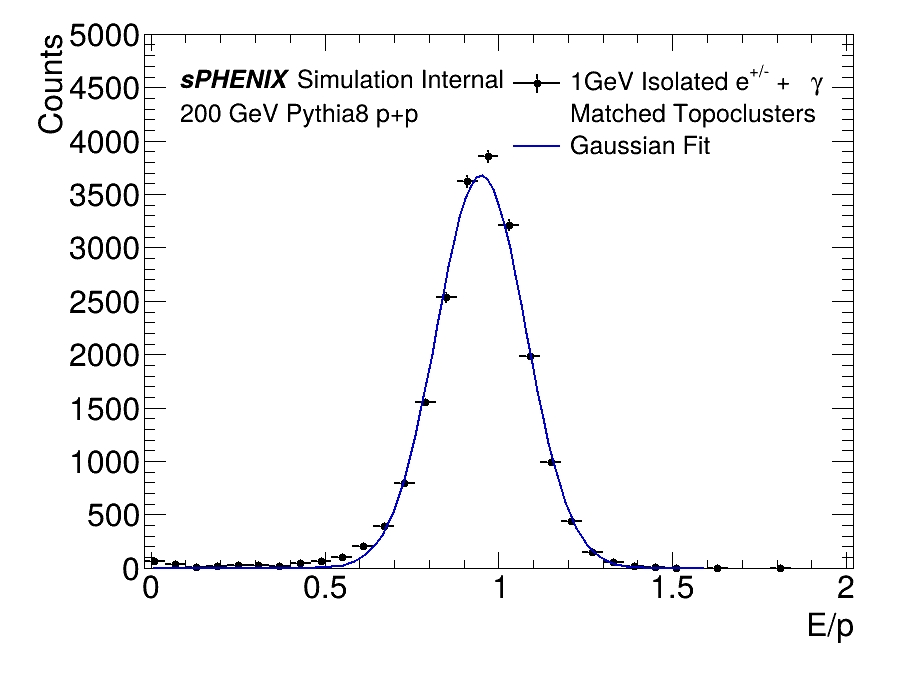
\includegraphics[width=\textwidth]{figures/chapter5/EM_Isolated_Resolution_3Plots_sphenix.png}
    \caption{EM particles ($E>1$\,GeV, $\Delta R<0.1$)}
  \end{subfigure}
  \hfill
  \begin{subfigure}[b]{0.48\textwidth}
    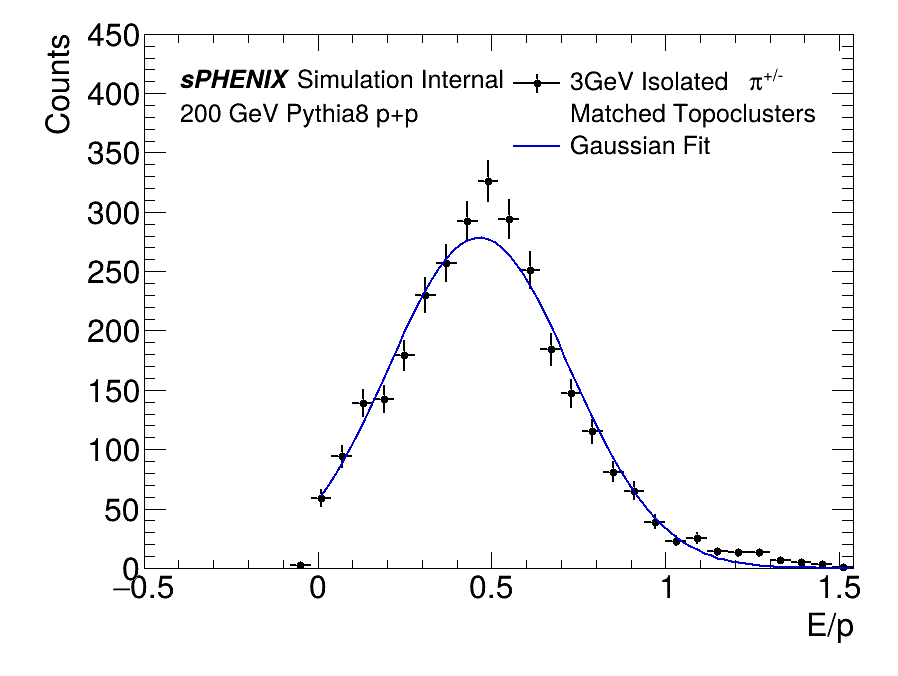
\includegraphics[width=\textwidth]{figures/chapter5/Hadron_Isolated_Resolution_3Plots_sphenix.png}
    \caption{Hadronic particles ($E>3$\,GeV, $\Delta R<0.2$)}
  \end{subfigure}
  \caption{$E/p$ distributions from isolated single hadrons in \pythia simulation with realistic pedestal noise conditions from the Run 2024 p+p collision period. Distributions for EM (left) and hadronic (right) particles using $\langle3\sigma_{ped}\rangle$ topocluster noise thresholds.}
  \label{fig:topocluster_resolution_3sigma}
\end{figure}

Additional studies were performed for lower energy hadrons with $E < 1$ GeV and matched within $\Delta R < 0.2$.
However for lower energy particles, the magnetic field effects become more significant and the matching between truth particles and topoclusters becomes more difficult.
A short study was performed studying the resolution of hadronic particles with $E < 1$ GeV and matched within $\Delta R < 0.2$ to tracks and the track projection module was used to match these tracks to the topoclusters.
These lower energy hadron simulation studies are included in Appendix~\ref{sec:additional_topo_reso}.

\subsection{Reconstructed UE Energy from towers versus topoclusters}

The underlying event measurement is defined as the average total transverse energy density ($\langle\Sigma E_{T}/\delta\eta\delta\phi\rangle$) in the transverse region of jet events. 
This observable is calculated at the reconstruction level by first summing the total transverse energy ($E_{T}$) from either calorimeter towers or calorimeter clusters in the transverse region. 

The total transverse energy ($\Sigma E_{T}$) is then averaged over all jet events for a particular jet $p_{T}$, giving the average total transverse energy, $\langle\Sigma E_{T}\rangle$ in the transverse region. Finally, the average transverse energy density ($\langle\Sigma E_{T}/\delta\eta\delta\phi\rangle$) is calculated by dividing by the overall acceptance in the transverse region in $\eta$ and $\phi$. The acceptance of the transverse region is $\Delta\eta = 2.2$ x $\Delta\phi = 2\pi /3$. 

The reconstructed transverse energy in dijet events from summing calorimeter towers versus summing topoclusters are shown in Figure~\ref{fig:towers_and_topo} with the $\langle3\sigma_{ped}\rangle$ noise thresholds for the topocluster construction. 
The \ET{} distribution from towers is wider than the distribution from topoclusters.
Notably, the mean topocluster \ET{} in the transverse region is about half the tower sum \ET{} in the transverse region, meaning likely the towers measurement contains a large noise contribution. 
This theory that the towers measurement includes contributions from noise is supported by the results in Section~\ref{sec:ueinpp_runbyrunqa}, which includes studies of the mean topocluster and tower total \ET{} under varying noise conditions.
Therefore, the robustness of the topoclusters to noise makes using the topoclusters with optimized noise thresholds the best choice for this measurement. 

\begin{figure}
    \centering
    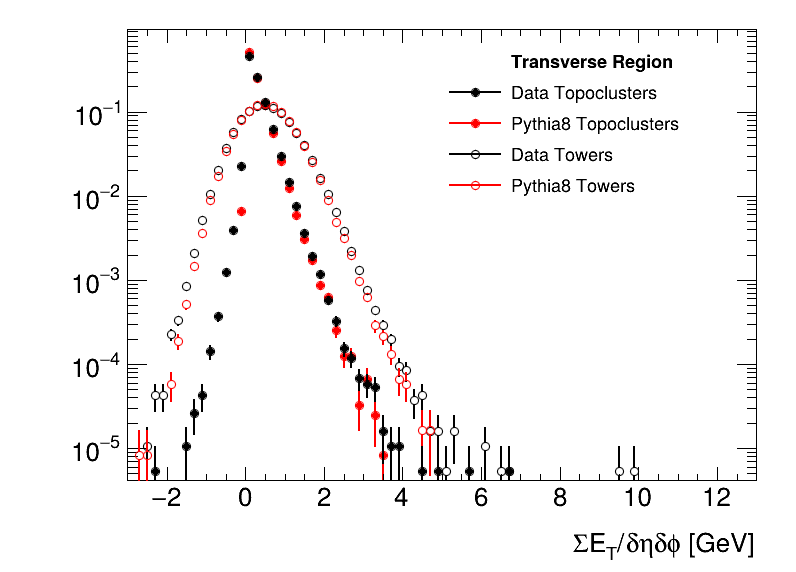
\includegraphics[width=0.7\linewidth]{figures/chapter5/h_ue_transverse_Topoclusters.png}
    \caption{Comparison of transverse region energy distributions from topoclusters (solid points) and towers (hollow points) in dijet events in data (black) and Pythia8 p+p simulation (red).}
    \label{fig:towers_and_topo}
\end{figure}